\documentclass[tikz,border=4pt]{standalone}
\usepackage{amsmath}
\usepackage{xcolor}
\usetikzlibrary{calc}

\tikzset{
  wire/.style={draw=black, line width=0.55pt},
  guide/.style={draw=black, dashed, line width=0.45pt},
  block/.style={
    draw=black,
    fill=white,
    line width=0.6pt,
    minimum width=1.95cm,
    minimum height=1.22cm,
    align=center,
    inner sep=2pt
  },
  feature/.style={
    draw=black,
    fill=white,
    line width=0.55pt,
    minimum width=0.18cm,
    minimum height=1.08cm,
    inner sep=0pt
  },
  smalllabel/.style={font=\footnotesize},
  mathlabel/.style={font=\large}
}

\begin{document}
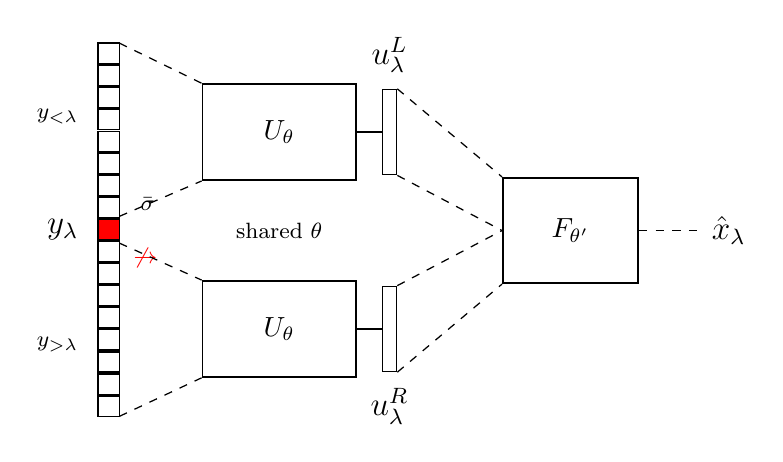
\begin{tikzpicture}
  % Spectrum strip: the red center pixel is the held-out target.
  \foreach \i in {0,...,7} {
    \pgfmathsetmacro{\ytop}{2.38 - 0.28*\i}
    \draw[wire, fill=white] (-4.95,\ytop) rectangle (-4.68,\ytop-0.26);
  }
  \draw[wire, fill=red] (-4.95,0.14) rectangle (-4.68,-0.12);
  \foreach \i in {9,...,16} {
    \pgfmathsetmacro{\ytop}{2.38 - 0.28*\i}
    \draw[wire, fill=white] (-4.95,\ytop) rectangle (-4.68,\ytop-0.26);
  }

  \node[mathlabel, anchor=east] at (-5.08,0.01) {$y_\lambda$};
  \node[smalllabel, anchor=east] at (-5.08,1.45) {$y_{<\lambda}$};
  \node[smalllabel, anchor=east] at (-5.08,-1.45) {$y_{>\lambda}$};
  \node[smalllabel] at (-4.32,0.34) {$\bar{\sigma}$};
  \node[smalllabel] at (-4.35,-0.35) {\textcolor{red}{$\not\to$}};

  \node[block] (UL) at (-2.65,1.25) {$U_\theta$};
  \node[block] (UR) at (-2.65,-1.25) {$U_\theta$};
  \node[smalllabel] at (-2.65,0) {shared $\theta$};

  \draw[guide] (-4.68,2.38) -- (UL.north west);
  \draw[guide] (-4.68,0.18) -- (UL.south west);
  \draw[guide] (-4.68,-0.16) -- (UR.north west);
  \draw[guide] (-4.68,-2.36) -- (UR.south west);

  \node[feature] (FL) at (-1.25,1.25) {};
  \node[feature] (FR) at (-1.25,-1.25) {};
  \node[mathlabel, anchor=south] at (-1.25,1.88) {$u_\lambda^{L}$};
  \node[mathlabel, anchor=north] at (-1.25,-1.88) {$u_\lambda^{R}$};

  \draw[wire] (UL.east) -- (FL.west);
  \draw[wire] (UR.east) -- (FR.west);

  \node[block, minimum width=1.72cm, minimum height=1.34cm] (F) at (1.05,0) {$F_{\theta'}$};
  \draw[guide] (FL.north east) -- (F.north west);
  \draw[guide] (FL.south east) -- (F.west);
  \draw[guide] (FR.north east) -- (F.west);
  \draw[guide] (FR.south east) -- (F.south west);

  \draw[guide] (F.east) -- (2.72,0);
  \node[mathlabel, anchor=west] at (2.72,0) {$\hat{x}_\lambda$};
\end{tikzpicture}
\end{document}
